\documentclass{standalone}
\usepackage{tikz}
\usetikzlibrary{patterns}
\usetikzlibrary{positioning}
\usetikzlibrary{patterns, positioning}
\usetikzlibrary{shapes.misc}
\usepackage[outline]{contour}
\contourlength{1.5pt} 
\usetikzlibrary{calc}
        \usepackage{relsize}
        \tikzset{fontscale/.style = {font=\relsize{#1}}}

\begin{document}
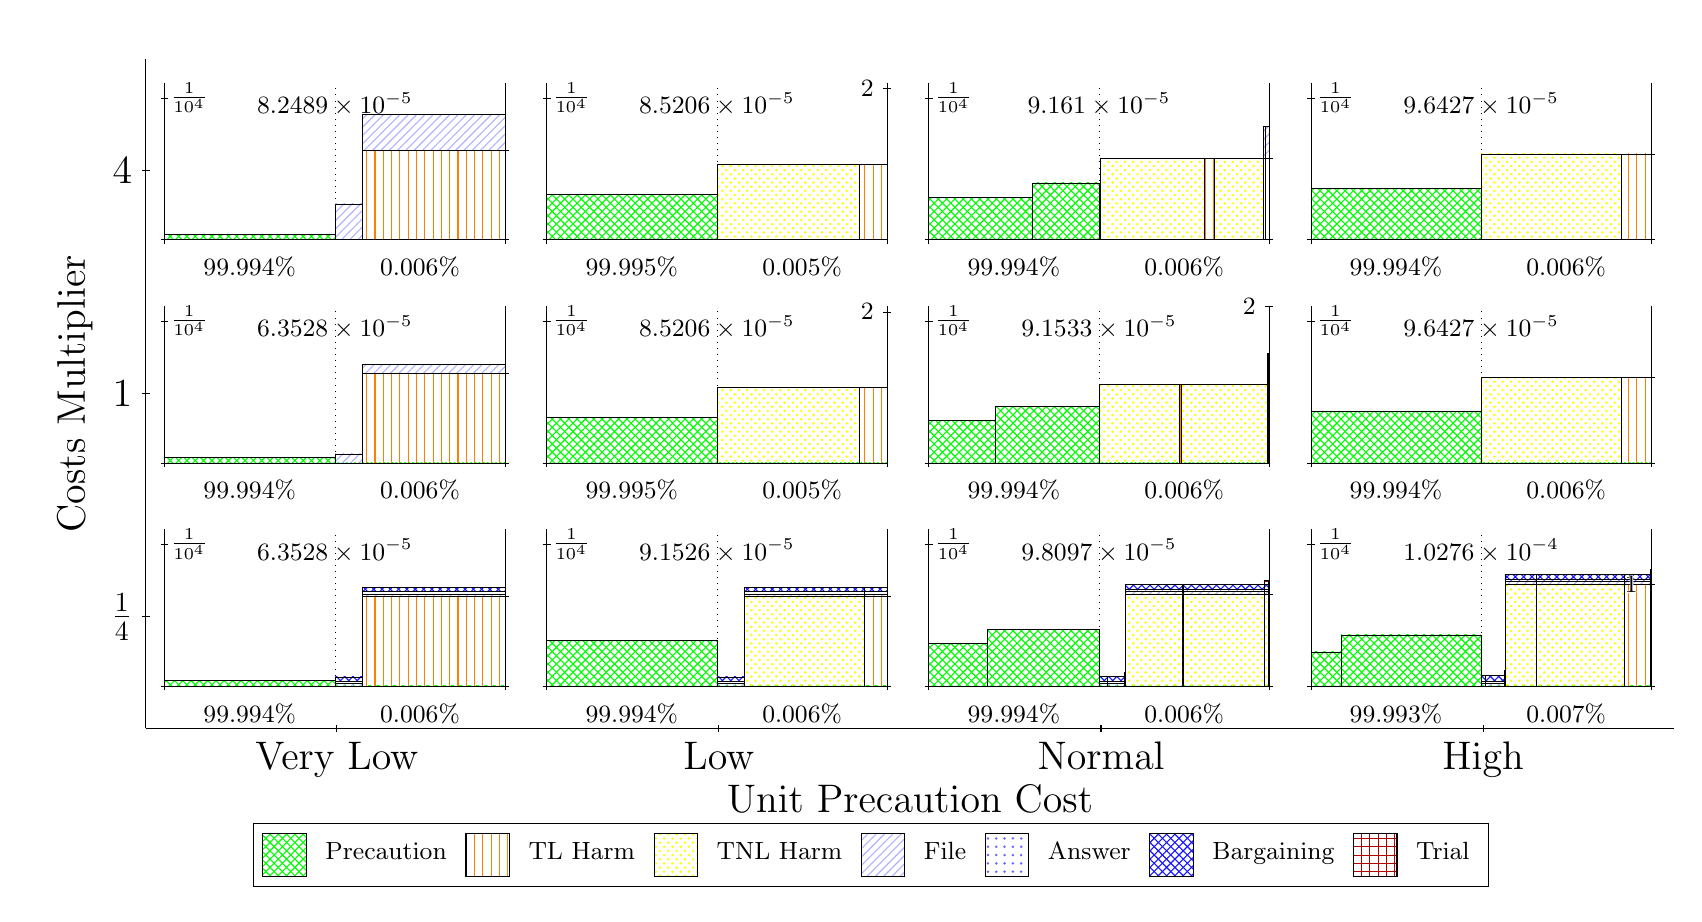
\begin{tikzpicture}
\clip(-0.5,-1.1) rectangle +(20.91,11);
\draw[black] (1,1) -- (1,9.5);
\node[rotate=90, fontscale=2, anchor=center] at (0.1, 5.25) {Costs Multiplier};
\draw[black] (0.95,2.4167) -- (1.05,2.4167);
\node[fontscale=2, anchor=east] at (0.95, 2.4167) {$\frac{1}{4}$};
\draw[black] (0.95,5.25) -- (1.05,5.25);
\node[fontscale=2, anchor=east] at (0.95, 5.25) {1};
\draw[black] (0.95,8.0833) -- (1.05,8.0833);
\node[fontscale=2, anchor=east] at (0.95, 8.0833) {4};

\draw[black] (1,1) -- (20.41,1);
\node[fontscale=2, anchor=center] at (10.705, 0.1) {Unit Precaution Cost};
\draw[black] (3.4263,0.95) -- (3.4263,1.05);
\node[fontscale=2, anchor=north] at (3.4263, 0.95) {Very Low};
\draw[black] (8.2788,0.95) -- (8.2788,1.05);
\node[fontscale=2, anchor=north] at (8.2788, 0.95) {Low};
\draw[black] (13.131,0.95) -- (13.131,1.05);
\node[fontscale=2, anchor=north] at (13.131, 0.95) {Normal};
\draw[black] (17.984,0.95) -- (17.984,1.05);
\node[fontscale=2, anchor=north] at (17.984, 0.95) {High};


\draw[pattern=crosshatch, pattern color=green,draw=black,very thin] (1.2381,1.54) rectangle (3.4013,1.6121);
\draw[pattern=crosshatch, pattern color=green,draw=black,very thin] (3.4013,1.54) rectangle (3.7435,1.54);
\draw[pattern=north east lines, pattern color=blue!30,draw=black,very thin] (3.4013,1.54) rectangle (3.7435,1.5685);
\draw[pattern=dots,  pattern color=blue!60,draw=black,very thin] (3.4013,1.5685) rectangle (3.7435,1.597);
\draw[pattern=crosshatch,      pattern color=blue!90,draw=black,very thin] (3.4013,1.597) rectangle (3.7435,1.6539);
\draw[pattern=crosshatch, pattern color=green,draw=black,very thin] (3.7435,1.54) rectangle (5.5644,1.54);
\draw[pattern=vertical lines, pattern color=orange,draw=black,very thin] (3.7435,1.54) rectangle (5.5644,2.679);
\draw[pattern=north east lines, pattern color=blue!30,draw=black,very thin] (3.7435,2.679) rectangle (5.5644,2.7075);
\draw[pattern=dots,  pattern color=blue!60,draw=black,very thin] (3.7435,2.7075) rectangle (5.5644,2.736);
\draw[pattern=crosshatch,      pattern color=blue!90,draw=black,very thin] (3.7435,2.736) rectangle (5.5644,2.793);
\node[font=\small,text=black,anchor=north] at (3.4013, 3.5333) {$6.3528\times 10^{-5}$};
\draw[black,very thin] (1.2381,1.54) -- (1.2381,3.5333);
\draw[black,very thin] (1.1881,1.54) -- (1.2881,1.54);
\node[font=\small,text=black, anchor=west] at (1.1881, 1.54) {};
\draw[black,very thin] (1.1881,3.342) -- (1.2881,3.342);
\node[font=\small,text=black, anchor=west] at (1.1881, 3.342) {$\frac{1}{10^{4}}$};

\draw[black,dotted,very thin] (3.4013,1.5998) -- (3.4013,3.4735);
\draw[black,very thin] (5.5644,1.54) -- (5.5644,3.5333);
\draw[black,very thin] (5.5144,1.54) -- (5.6144,1.54);
\node[font=\small,text=black, anchor=east] at (5.5144, 1.54) {\contour{white}{}};
\draw[black,very thin] (5.5144,2.679) -- (5.6144,2.679);
\node[font=\small,text=black, anchor=east] at (5.5144, 2.679) {\contour{white}{}};

\draw[black,very thin] (1.2381,1.54) -- (5.5644,1.54);
\draw[black,very thin] (1.2381,1.49) -- (1.2381,1.59);
\node[font=\small,text=black, anchor=north] at (1.2381, 1.49) {};
\draw[black,very thin] (5.5644,1.49) -- (5.5644,1.59);
\node[font=\small,text=black, anchor=north] at (5.5644, 1.49) {};

\node[font=\small,text=black,anchor=south] at (2.3197, 0.94) {99.994\%};
\node[font=\small,text=black,anchor=south] at (4.4828, 0.94) {0.006\%};

\draw[pattern=crosshatch, pattern color=green,draw=black,very thin] (6.0906,1.54) rectangle (8.2538,2.1166);
\draw[pattern=crosshatch, pattern color=green,draw=black,very thin] (8.2538,1.54) rectangle (8.596,1.54);
\draw[pattern=north east lines, pattern color=blue!30,draw=black,very thin] (8.2538,1.54) rectangle (8.596,1.5685);
\draw[pattern=dots,  pattern color=blue!60,draw=black,very thin] (8.2538,1.5685) rectangle (8.596,1.597);
\draw[pattern=crosshatch,      pattern color=blue!90,draw=black,very thin] (8.2538,1.597) rectangle (8.596,1.6539);
\draw[pattern=crosshatch, pattern color=green,draw=black,very thin] (8.596,1.54) rectangle (10.121,1.54);
\draw[pattern=crosshatch dots, pattern color=yellow,draw=black,very thin] (8.596,1.54) rectangle (10.121,2.6791);
\draw[pattern=north east lines, pattern color=blue!30,draw=black,very thin] (8.596,2.6791) rectangle (10.121,2.7075);
\draw[pattern=dots,  pattern color=blue!60,draw=black,very thin] (8.596,2.7075) rectangle (10.121,2.736);
\draw[pattern=crosshatch,      pattern color=blue!90,draw=black,very thin] (8.596,2.736) rectangle (10.121,2.793);
\draw[pattern=crosshatch, pattern color=green,draw=black,very thin] (10.121,1.54) rectangle (10.417,1.54);
\draw[pattern=vertical lines, pattern color=orange,draw=black,very thin] (10.121,1.54) rectangle (10.417,2.6791);
\draw[pattern=north east lines, pattern color=blue!30,draw=black,very thin] (10.121,2.6791) rectangle (10.417,2.7075);
\draw[pattern=dots,  pattern color=blue!60,draw=black,very thin] (10.121,2.7075) rectangle (10.417,2.736);
\draw[pattern=crosshatch,      pattern color=blue!90,draw=black,very thin] (10.121,2.736) rectangle (10.417,2.793);
\node[font=\small,text=black,anchor=north] at (8.2538, 3.5333) {$9.1526\times 10^{-5}$};
\draw[black,very thin] (6.0906,1.54) -- (6.0906,3.5333);
\draw[black,very thin] (6.0406,1.54) -- (6.1406,1.54);
\node[font=\small,text=black, anchor=west] at (6.0406, 1.54) {};
\draw[black,very thin] (6.0406,3.342) -- (6.1406,3.342);
\node[font=\small,text=black, anchor=west] at (6.0406, 3.342) {$\frac{1}{10^{4}}$};

\draw[black,dotted,very thin] (8.2538,1.5998) -- (8.2538,3.4735);
\draw[black,very thin] (10.417,1.54) -- (10.417,3.5333);
\draw[black,very thin] (10.367,1.54) -- (10.467,1.54);
\node[font=\small,text=black, anchor=east] at (10.367, 1.54) {\contour{white}{}};
\draw[black,very thin] (10.367,2.679) -- (10.467,2.679);
\node[font=\small,text=black, anchor=east] at (10.367, 2.679) {\contour{white}{}};

\draw[black,very thin] (6.0906,1.54) -- (10.417,1.54);
\draw[black,very thin] (6.0906,1.49) -- (6.0906,1.59);
\node[font=\small,text=black, anchor=north] at (6.0906, 1.49) {};
\draw[black,very thin] (10.417,1.49) -- (10.417,1.59);
\node[font=\small,text=black, anchor=north] at (10.417, 1.49) {};

\node[font=\small,text=black,anchor=south] at (7.1722, 0.94) {99.994\%};
\node[font=\small,text=black,anchor=south] at (9.3353, 0.94) {0.006\%};

\draw[pattern=crosshatch, pattern color=green,draw=black,very thin] (10.943,1.54) rectangle (11.692,2.0806);
\draw[pattern=crosshatch, pattern color=green,draw=black,very thin] (11.692,1.54) rectangle (13.106,2.2608);
\draw[pattern=crosshatch, pattern color=green,draw=black,very thin] (13.106,1.54) rectangle (13.21,1.54);
\draw[pattern=north east lines, pattern color=blue!30,draw=black,very thin] (13.106,1.54) rectangle (13.21,1.5693);
\draw[pattern=dots,  pattern color=blue!60,draw=black,very thin] (13.106,1.5693) rectangle (13.21,1.5986);
\draw[pattern=crosshatch,      pattern color=blue!90,draw=black,very thin] (13.106,1.5986) rectangle (13.21,1.6571);
\draw[pattern=crosshatch, pattern color=green,draw=black,very thin] (13.21,1.54) rectangle (13.428,1.54);
\draw[pattern=north east lines, pattern color=blue!30,draw=black,very thin] (13.21,1.54) rectangle (13.428,1.5693);
\draw[pattern=dots,  pattern color=blue!60,draw=black,very thin] (13.21,1.5693) rectangle (13.428,1.5986);
\draw[pattern=crosshatch,      pattern color=blue!90,draw=black,very thin] (13.21,1.5986) rectangle (13.428,1.6571);
\draw[pattern=crosshatch, pattern color=green,draw=black,very thin] (13.428,1.54) rectangle (13.439,1.54);
\draw[pattern=north east lines, pattern color=blue!30,draw=black,very thin] (13.428,1.54) rectangle (13.439,1.5693);
\draw[pattern=dots,  pattern color=blue!60,draw=black,very thin] (13.428,1.5693) rectangle (13.439,1.5986);
\draw[pattern=crosshatch,      pattern color=blue!90,draw=black,very thin] (13.428,1.5986) rectangle (13.439,1.6571);
\draw[pattern=grid,            pattern color=red!70!black,draw=black,very thin] (13.428,1.6571) rectangle (13.439,1.7156);
\draw[pattern=crosshatch, pattern color=green,draw=black,very thin] (13.439,1.54) rectangle (14.165,1.54);
\draw[pattern=crosshatch dots, pattern color=yellow,draw=black,very thin] (13.439,1.54) rectangle (14.165,2.7104);
\draw[pattern=north east lines, pattern color=blue!30,draw=black,very thin] (13.439,2.7104) rectangle (14.165,2.7396);
\draw[pattern=dots,  pattern color=blue!60,draw=black,very thin] (13.439,2.7396) rectangle (14.165,2.7689);
\draw[pattern=crosshatch,      pattern color=blue!90,draw=black,very thin] (13.439,2.7689) rectangle (14.165,2.8274);
\draw[pattern=crosshatch, pattern color=green,draw=black,very thin] (14.165,1.54) rectangle (14.171,1.54);
\draw[pattern=vertical lines, pattern color=orange,draw=black,very thin] (14.165,1.54) rectangle (14.171,2.7104);
\draw[pattern=north east lines, pattern color=blue!30,draw=black,very thin] (14.165,2.7104) rectangle (14.171,2.7396);
\draw[pattern=dots,  pattern color=blue!60,draw=black,very thin] (14.165,2.7396) rectangle (14.171,2.7689);
\draw[pattern=crosshatch,      pattern color=blue!90,draw=black,very thin] (14.165,2.7689) rectangle (14.171,2.8274);
\draw[pattern=crosshatch, pattern color=green,draw=black,very thin] (14.171,1.54) rectangle (15.2,1.54);
\draw[pattern=crosshatch dots, pattern color=yellow,draw=black,very thin] (14.171,1.54) rectangle (15.2,2.7104);
\draw[pattern=north east lines, pattern color=blue!30,draw=black,very thin] (14.171,2.7104) rectangle (15.2,2.7396);
\draw[pattern=dots,  pattern color=blue!60,draw=black,very thin] (14.171,2.7396) rectangle (15.2,2.7689);
\draw[pattern=crosshatch,      pattern color=blue!90,draw=black,very thin] (14.171,2.7689) rectangle (15.2,2.8274);
\draw[pattern=crosshatch, pattern color=green,draw=black,very thin] (15.2,1.54) rectangle (15.252,1.54);
\draw[pattern=crosshatch dots, pattern color=yellow,draw=black,very thin] (15.2,1.54) rectangle (15.252,2.7104);
\draw[pattern=north east lines, pattern color=blue!30,draw=black,very thin] (15.2,2.7104) rectangle (15.252,2.7396);
\draw[pattern=dots,  pattern color=blue!60,draw=black,very thin] (15.2,2.7396) rectangle (15.252,2.7689);
\draw[pattern=crosshatch,      pattern color=blue!90,draw=black,very thin] (15.2,2.7689) rectangle (15.252,2.8274);
\draw[pattern=grid,            pattern color=red!70!black,draw=black,very thin] (15.2,2.8274) rectangle (15.252,2.8859);
\draw[pattern=crosshatch, pattern color=green,draw=black,very thin] (15.252,1.54) rectangle (15.269,1.54);
\draw[pattern=vertical lines, pattern color=orange,draw=black,very thin] (15.252,1.54) rectangle (15.269,2.7104);
\draw[pattern=north east lines, pattern color=blue!30,draw=black,very thin] (15.252,2.7104) rectangle (15.269,2.7396);
\draw[pattern=dots,  pattern color=blue!60,draw=black,very thin] (15.252,2.7396) rectangle (15.269,2.7689);
\draw[pattern=crosshatch,      pattern color=blue!90,draw=black,very thin] (15.252,2.7689) rectangle (15.269,2.8274);
\draw[pattern=grid,            pattern color=red!70!black,draw=black,very thin] (15.252,2.8274) rectangle (15.269,2.8859);
\node[font=\small,text=black,anchor=north] at (13.106, 3.5333) {$9.8097\times 10^{-5}$};
\draw[black,very thin] (10.943,1.54) -- (10.943,3.5333);
\draw[black,very thin] (10.893,1.54) -- (10.993,1.54);
\node[font=\small,text=black, anchor=west] at (10.893, 1.54) {};
\draw[black,very thin] (10.893,3.342) -- (10.993,3.342);
\node[font=\small,text=black, anchor=west] at (10.893, 3.342) {$\frac{1}{10^{4}}$};

\draw[black,dotted,very thin] (13.106,1.5998) -- (13.106,3.4735);
\draw[black,very thin] (15.269,1.54) -- (15.269,3.5333);
\draw[black,very thin] (15.219,1.54) -- (15.319,1.54);
\node[font=\small,text=black, anchor=east] at (15.219, 1.54) {\contour{white}{}};
\draw[black,very thin] (15.219,2.7103) -- (15.319,2.7103);
\node[font=\small,text=black, anchor=east] at (15.219, 2.7103) {\contour{white}{}};

\draw[black,very thin] (10.943,1.54) -- (15.269,1.54);
\draw[black,very thin] (10.943,1.49) -- (10.943,1.59);
\node[font=\small,text=black, anchor=north] at (10.943, 1.49) {};
\draw[black,very thin] (15.269,1.49) -- (15.269,1.59);
\node[font=\small,text=black, anchor=north] at (15.269, 1.49) {};

\node[font=\small,text=black,anchor=south] at (12.025, 0.94) {99.994\%};
\node[font=\small,text=black,anchor=south] at (14.188, 0.94) {0.006\%};

\draw[pattern=crosshatch, pattern color=green,draw=black,very thin] (15.796,1.54) rectangle (16.177,1.9725);
\draw[pattern=crosshatch, pattern color=green,draw=black,very thin] (16.177,1.54) rectangle (17.959,2.1887);
\draw[pattern=crosshatch, pattern color=green,draw=black,very thin] (17.959,1.54) rectangle (18.009,1.54);
\draw[pattern=north east lines, pattern color=blue!30,draw=black,very thin] (17.959,1.54) rectangle (18.009,1.5723);
\draw[pattern=dots,  pattern color=blue!60,draw=black,very thin] (17.959,1.5723) rectangle (18.009,1.6046);
\draw[pattern=crosshatch,      pattern color=blue!90,draw=black,very thin] (17.959,1.6046) rectangle (18.009,1.6692);
\draw[pattern=crosshatch, pattern color=green,draw=black,very thin] (18.009,1.54) rectangle (18.258,1.54);
\draw[pattern=north east lines, pattern color=blue!30,draw=black,very thin] (18.009,1.54) rectangle (18.258,1.5723);
\draw[pattern=dots,  pattern color=blue!60,draw=black,very thin] (18.009,1.5723) rectangle (18.258,1.6046);
\draw[pattern=crosshatch,      pattern color=blue!90,draw=black,very thin] (18.009,1.6046) rectangle (18.258,1.6692);
\draw[pattern=crosshatch, pattern color=green,draw=black,very thin] (18.258,1.54) rectangle (18.261,1.54);
\draw[pattern=north east lines, pattern color=blue!30,draw=black,very thin] (18.258,1.54) rectangle (18.261,1.5723);
\draw[pattern=dots,  pattern color=blue!60,draw=black,very thin] (18.258,1.5723) rectangle (18.261,1.6046);
\draw[pattern=crosshatch,      pattern color=blue!90,draw=black,very thin] (18.258,1.6046) rectangle (18.261,1.6692);
\draw[pattern=grid,            pattern color=red!70!black,draw=black,very thin] (18.258,1.6692) rectangle (18.261,1.7338);
\draw[pattern=crosshatch, pattern color=green,draw=black,very thin] (18.261,1.54) rectangle (18.658,1.54);
\draw[pattern=crosshatch dots, pattern color=yellow,draw=black,very thin] (18.261,1.54) rectangle (18.658,2.8316);
\draw[pattern=north east lines, pattern color=blue!30,draw=black,very thin] (18.261,2.8316) rectangle (18.658,2.8639);
\draw[pattern=dots,  pattern color=blue!60,draw=black,very thin] (18.261,2.8639) rectangle (18.658,2.8962);
\draw[pattern=crosshatch,      pattern color=blue!90,draw=black,very thin] (18.261,2.8962) rectangle (18.658,2.9608);
\draw[pattern=crosshatch, pattern color=green,draw=black,very thin] (18.658,1.54) rectangle (18.659,1.54);
\draw[pattern=vertical lines, pattern color=orange,draw=black,very thin] (18.658,1.54) rectangle (18.659,2.8316);
\draw[pattern=north east lines, pattern color=blue!30,draw=black,very thin] (18.658,2.8316) rectangle (18.659,2.8639);
\draw[pattern=dots,  pattern color=blue!60,draw=black,very thin] (18.658,2.8639) rectangle (18.659,2.8962);
\draw[pattern=crosshatch,      pattern color=blue!90,draw=black,very thin] (18.658,2.8962) rectangle (18.659,2.9608);
\draw[pattern=crosshatch, pattern color=green,draw=black,very thin] (18.659,1.54) rectangle (19.778,1.54);
\draw[pattern=crosshatch dots, pattern color=yellow,draw=black,very thin] (18.659,1.54) rectangle (19.778,2.8317);
\draw[pattern=north east lines, pattern color=blue!30,draw=black,very thin] (18.659,2.8317) rectangle (19.778,2.8639);
\draw[pattern=dots,  pattern color=blue!60,draw=black,very thin] (18.659,2.8639) rectangle (19.778,2.8962);
\draw[pattern=crosshatch,      pattern color=blue!90,draw=black,very thin] (18.659,2.8962) rectangle (19.778,2.9608);
\draw[pattern=crosshatch, pattern color=green,draw=black,very thin] (19.778,1.54) rectangle (20.101,1.54);
\draw[pattern=vertical lines, pattern color=orange,draw=black,very thin] (19.778,1.54) rectangle (20.101,2.8317);
\draw[pattern=north east lines, pattern color=blue!30,draw=black,very thin] (19.778,2.8317) rectangle (20.101,2.8639);
\draw[pattern=dots,  pattern color=blue!60,draw=black,very thin] (19.778,2.8639) rectangle (20.101,2.8962);
\draw[pattern=crosshatch,      pattern color=blue!90,draw=black,very thin] (19.778,2.8962) rectangle (20.101,2.9608);
\draw[pattern=crosshatch, pattern color=green,draw=black,very thin] (20.101,1.54) rectangle (20.12,1.54);
\draw[pattern=crosshatch dots, pattern color=yellow,draw=black,very thin] (20.101,1.54) rectangle (20.12,2.8316);
\draw[pattern=north east lines, pattern color=blue!30,draw=black,very thin] (20.101,2.8316) rectangle (20.12,2.8639);
\draw[pattern=dots,  pattern color=blue!60,draw=black,very thin] (20.101,2.8639) rectangle (20.12,2.8962);
\draw[pattern=crosshatch,      pattern color=blue!90,draw=black,very thin] (20.101,2.8962) rectangle (20.12,2.9608);
\draw[pattern=grid,            pattern color=red!70!black,draw=black,very thin] (20.101,2.9608) rectangle (20.12,3.0254);
\draw[pattern=crosshatch, pattern color=green,draw=black,very thin] (20.12,1.54) rectangle (20.122,1.54);
\draw[pattern=vertical lines, pattern color=orange,draw=black,very thin] (20.12,1.54) rectangle (20.122,2.8316);
\draw[pattern=north east lines, pattern color=blue!30,draw=black,very thin] (20.12,2.8316) rectangle (20.122,2.8639);
\draw[pattern=dots,  pattern color=blue!60,draw=black,very thin] (20.12,2.8639) rectangle (20.122,2.8962);
\draw[pattern=crosshatch,      pattern color=blue!90,draw=black,very thin] (20.12,2.8962) rectangle (20.122,2.9608);
\draw[pattern=grid,            pattern color=red!70!black,draw=black,very thin] (20.12,2.9608) rectangle (20.122,3.0254);
\node[font=\small,text=black,anchor=north] at (17.959, 3.5333) {$1.0276\times 10^{-4}$};
\draw[black,very thin] (15.796,1.54) -- (15.796,3.5333);
\draw[black,very thin] (15.746,1.54) -- (15.846,1.54);
\node[font=\small,text=black, anchor=west] at (15.746, 1.54) {};
\draw[black,very thin] (15.746,3.342) -- (15.846,3.342);
\node[font=\small,text=black, anchor=west] at (15.746, 3.342) {$\frac{1}{10^{4}}$};

\draw[black,dotted,very thin] (17.959,1.5998) -- (17.959,3.4735);
\draw[black,very thin] (20.122,1.54) -- (20.122,3.5333);
\draw[black,very thin] (20.072,1.54) -- (20.172,1.54);
\node[font=\small,text=black, anchor=east] at (20.072, 1.54) {\contour{white}{}};
\draw[black,very thin] (20.072,2.8316) -- (20.172,2.8316);
\node[font=\small,text=black, anchor=east] at (20.072, 2.8316) {\contour{white}{1}};

\draw[black,very thin] (15.796,1.54) -- (20.122,1.54);
\draw[black,very thin] (15.796,1.49) -- (15.796,1.59);
\node[font=\small,text=black, anchor=north] at (15.796, 1.49) {};
\draw[black,very thin] (20.122,1.49) -- (20.122,1.59);
\node[font=\small,text=black, anchor=north] at (20.122, 1.49) {};

\node[font=\small,text=black,anchor=south] at (16.877, 0.94) {99.993\%};
\node[font=\small,text=black,anchor=south] at (19.04, 0.94) {0.007\%};

\draw[pattern=crosshatch, pattern color=green,draw=black,very thin] (1.2381,4.3733) rectangle (3.4013,4.4454);
\draw[pattern=crosshatch, pattern color=green,draw=black,very thin] (3.4013,4.3733) rectangle (3.7435,4.3733);
\draw[pattern=north east lines, pattern color=blue!30,draw=black,very thin] (3.4013,4.3733) rectangle (3.7435,4.4872);
\draw[pattern=crosshatch, pattern color=green,draw=black,very thin] (3.7435,4.3733) rectangle (5.5644,4.3733);
\draw[pattern=vertical lines, pattern color=orange,draw=black,very thin] (3.7435,4.3733) rectangle (5.5644,5.5124);
\draw[pattern=north east lines, pattern color=blue!30,draw=black,very thin] (3.7435,5.5124) rectangle (5.5644,5.6263);
\node[font=\small,text=black,anchor=north] at (3.4013, 6.3667) {$6.3528\times 10^{-5}$};
\draw[black,very thin] (1.2381,4.3733) -- (1.2381,6.3667);
\draw[black,very thin] (1.1881,4.3733) -- (1.2881,4.3733);
\node[font=\small,text=black, anchor=west] at (1.1881, 4.3733) {};
\draw[black,very thin] (1.1881,6.1753) -- (1.2881,6.1753);
\node[font=\small,text=black, anchor=west] at (1.1881, 6.1753) {$\frac{1}{10^{4}}$};

\draw[black,dotted,very thin] (3.4013,4.4331) -- (3.4013,6.3069);
\draw[black,very thin] (5.5644,4.3733) -- (5.5644,6.3667);
\draw[black,very thin] (5.5144,4.3733) -- (5.6144,4.3733);
\node[font=\small,text=black, anchor=east] at (5.5144, 4.3733) {\contour{white}{}};
\draw[black,very thin] (5.5144,5.5124) -- (5.6144,5.5124);
\node[font=\small,text=black, anchor=east] at (5.5144, 5.5124) {\contour{white}{}};

\draw[black,very thin] (1.2381,4.3733) -- (5.5644,4.3733);
\draw[black,very thin] (1.2381,4.3233) -- (1.2381,4.4233);
\node[font=\small,text=black, anchor=north] at (1.2381, 4.3233) {};
\draw[black,very thin] (5.5644,4.3233) -- (5.5644,4.4233);
\node[font=\small,text=black, anchor=north] at (5.5644, 4.3233) {};

\node[font=\small,text=black,anchor=south] at (2.3197, 3.7733) {99.994\%};
\node[font=\small,text=black,anchor=south] at (4.4828, 3.7733) {0.006\%};

\draw[pattern=crosshatch, pattern color=green,draw=black,very thin] (6.0906,4.3733) rectangle (8.2538,4.95);
\draw[pattern=crosshatch, pattern color=green,draw=black,very thin] (8.2538,4.3733) rectangle (10.066,4.3734);
\draw[pattern=crosshatch dots, pattern color=yellow,draw=black,very thin] (8.2538,4.3734) rectangle (10.066,5.3322);
\draw[pattern=crosshatch, pattern color=green,draw=black,very thin] (10.066,4.3733) rectangle (10.417,4.3734);
\draw[pattern=vertical lines, pattern color=orange,draw=black,very thin] (10.066,4.3734) rectangle (10.417,5.3322);
\node[font=\small,text=black,anchor=north] at (8.2538, 6.3667) {$8.5206\times 10^{-5}$};
\draw[black,very thin] (6.0906,4.3733) -- (6.0906,6.3667);
\draw[black,very thin] (6.0406,4.3733) -- (6.1406,4.3733);
\node[font=\small,text=black, anchor=west] at (6.0406, 4.3733) {};
\draw[black,very thin] (6.0406,6.1754) -- (6.1406,6.1754);
\node[font=\small,text=black, anchor=west] at (6.0406, 6.1754) {$\frac{1}{10^{4}}$};

\draw[black,dotted,very thin] (8.2538,4.4331) -- (8.2538,6.3069);
\draw[black,very thin] (10.417,4.3733) -- (10.417,6.3667);
\draw[black,very thin] (10.367,6.291) -- (10.467,6.291);
\node[font=\small,text=black, anchor=east] at (10.367, 6.291) {\contour{white}{2}};

\draw[black,very thin] (6.0906,4.3733) -- (10.417,4.3733);
\draw[black,very thin] (6.0906,4.3233) -- (6.0906,4.4233);
\node[font=\small,text=black, anchor=north] at (6.0906, 4.3233) {};
\draw[black,very thin] (10.417,4.3233) -- (10.417,4.4233);
\node[font=\small,text=black, anchor=north] at (10.417, 4.3233) {};

\node[font=\small,text=black,anchor=south] at (7.1722, 3.7733) {99.995\%};
\node[font=\small,text=black,anchor=south] at (9.3353, 3.7733) {0.005\%};

\draw[pattern=crosshatch, pattern color=green,draw=black,very thin] (10.943,4.3733) rectangle (11.791,4.9139);
\draw[pattern=crosshatch, pattern color=green,draw=black,very thin] (11.791,4.3733) rectangle (13.106,5.0941);
\draw[pattern=crosshatch, pattern color=green,draw=black,very thin] (13.106,4.3733) rectangle (13.109,4.3734);
\draw[pattern=north east lines, pattern color=blue!30,draw=black,very thin] (13.106,4.3734) rectangle (13.109,4.473);
\draw[pattern=dots,  pattern color=blue!60,draw=black,very thin] (13.106,4.473) rectangle (13.109,4.5726);
\draw[pattern=crosshatch,      pattern color=blue!90,draw=black,very thin] (13.106,4.5726) rectangle (13.109,4.7718);
\draw[pattern=crosshatch, pattern color=green,draw=black,very thin] (13.109,4.3733) rectangle (14.126,4.3734);
\draw[pattern=crosshatch dots, pattern color=yellow,draw=black,very thin] (13.109,4.3734) rectangle (14.126,5.3694);
\draw[pattern=crosshatch, pattern color=green,draw=black,very thin] (14.126,4.3733) rectangle (14.151,4.3734);
\draw[pattern=vertical lines, pattern color=orange,draw=black,very thin] (14.126,4.3734) rectangle (14.151,5.3694);
\draw[pattern=crosshatch, pattern color=green,draw=black,very thin] (14.151,4.3733) rectangle (15.249,4.3734);
\draw[pattern=crosshatch dots, pattern color=yellow,draw=black,very thin] (14.151,4.3734) rectangle (15.249,5.3694);
\draw[pattern=crosshatch, pattern color=green,draw=black,very thin] (15.249,4.3733) rectangle (15.256,4.3734);
\draw[pattern=crosshatch dots, pattern color=yellow,draw=black,very thin] (15.249,4.3734) rectangle (15.256,5.3694);
\draw[pattern=north east lines, pattern color=blue!30,draw=black,very thin] (15.249,5.3694) rectangle (15.256,5.469);
\draw[pattern=dots,  pattern color=blue!60,draw=black,very thin] (15.249,5.469) rectangle (15.256,5.5686);
\draw[pattern=crosshatch,      pattern color=blue!90,draw=black,very thin] (15.249,5.5686) rectangle (15.256,5.7678);
\draw[pattern=crosshatch, pattern color=green,draw=black,very thin] (15.256,4.3733) rectangle (15.266,4.3734);
\draw[pattern=vertical lines, pattern color=orange,draw=black,very thin] (15.256,4.3734) rectangle (15.266,5.3694);
\draw[pattern=north east lines, pattern color=blue!30,draw=black,very thin] (15.256,5.3694) rectangle (15.266,5.469);
\draw[pattern=dots,  pattern color=blue!60,draw=black,very thin] (15.256,5.469) rectangle (15.266,5.5686);
\draw[pattern=crosshatch,      pattern color=blue!90,draw=black,very thin] (15.256,5.5686) rectangle (15.266,5.7678);
\draw[pattern=crosshatch, pattern color=green,draw=black,very thin] (15.266,4.3733) rectangle (15.269,4.3734);
\draw[pattern=crosshatch dots, pattern color=yellow,draw=black,very thin] (15.266,4.3734) rectangle (15.269,5.3694);
\draw[pattern=north east lines, pattern color=blue!30,draw=black,very thin] (15.266,5.3694) rectangle (15.269,5.469);
\draw[pattern=dots,  pattern color=blue!60,draw=black,very thin] (15.266,5.469) rectangle (15.269,5.5686);
\draw[pattern=crosshatch,      pattern color=blue!90,draw=black,very thin] (15.266,5.5686) rectangle (15.269,5.7678);
\draw[pattern=grid,            pattern color=red!70!black,draw=black,very thin] (15.266,5.7678) rectangle (15.269,5.967);
\draw[pattern=crosshatch, pattern color=green,draw=black,very thin] (15.269,4.3733) rectangle (15.269,4.3734);
\draw[pattern=vertical lines, pattern color=orange,draw=black,very thin] (15.269,4.3734) rectangle (15.269,5.3694);
\draw[pattern=north east lines, pattern color=blue!30,draw=black,very thin] (15.269,5.3694) rectangle (15.269,5.469);
\draw[pattern=dots,  pattern color=blue!60,draw=black,very thin] (15.269,5.469) rectangle (15.269,5.5686);
\draw[pattern=crosshatch,      pattern color=blue!90,draw=black,very thin] (15.269,5.5686) rectangle (15.269,5.7678);
\draw[pattern=grid,            pattern color=red!70!black,draw=black,very thin] (15.269,5.7678) rectangle (15.269,5.967);
\node[font=\small,text=black,anchor=north] at (13.106, 6.3667) {$9.1533\times 10^{-5}$};
\draw[black,very thin] (10.943,4.3733) -- (10.943,6.3667);
\draw[black,very thin] (10.893,4.3733) -- (10.993,4.3733);
\node[font=\small,text=black, anchor=west] at (10.893, 4.3733) {};
\draw[black,very thin] (10.893,6.1753) -- (10.993,6.1753);
\node[font=\small,text=black, anchor=west] at (10.893, 6.1753) {$\frac{1}{10^{4}}$};

\draw[black,dotted,very thin] (13.106,4.4331) -- (13.106,6.3069);
\draw[black,very thin] (15.269,4.3733) -- (15.269,6.3667);
\draw[black,very thin] (15.219,6.3654) -- (15.319,6.3654);
\node[font=\small,text=black, anchor=east] at (15.219, 6.3654) {\contour{white}{2}};

\draw[black,very thin] (10.943,4.3733) -- (15.269,4.3733);
\draw[black,very thin] (10.943,4.3233) -- (10.943,4.4233);
\node[font=\small,text=black, anchor=north] at (10.943, 4.3233) {};
\draw[black,very thin] (15.269,4.3233) -- (15.269,4.4233);
\node[font=\small,text=black, anchor=north] at (15.269, 4.3233) {};

\node[font=\small,text=black,anchor=south] at (12.025, 3.7733) {99.994\%};
\node[font=\small,text=black,anchor=south] at (14.188, 3.7733) {0.006\%};

\draw[pattern=crosshatch, pattern color=green,draw=black,very thin] (15.796,4.3733) rectangle (17.959,5.0221);
\draw[pattern=crosshatch, pattern color=green,draw=black,very thin] (17.959,4.3733) rectangle (19.738,4.3734);
\draw[pattern=crosshatch dots, pattern color=yellow,draw=black,very thin] (17.959,4.3734) rectangle (19.738,5.4623);
\draw[pattern=crosshatch, pattern color=green,draw=black,very thin] (19.738,4.3733) rectangle (20.122,4.3734);
\draw[pattern=vertical lines, pattern color=orange,draw=black,very thin] (19.738,4.3734) rectangle (20.122,5.4623);
\node[font=\small,text=black,anchor=north] at (17.959, 6.3667) {$9.6427\times 10^{-5}$};
\draw[black,very thin] (15.796,4.3733) -- (15.796,6.3667);
\draw[black,very thin] (15.746,4.3733) -- (15.846,4.3733);
\node[font=\small,text=black, anchor=west] at (15.746, 4.3733) {};
\draw[black,very thin] (15.746,6.1753) -- (15.846,6.1753);
\node[font=\small,text=black, anchor=west] at (15.746, 6.1753) {$\frac{1}{10^{4}}$};

\draw[black,dotted,very thin] (17.959,4.4331) -- (17.959,6.3069);
\draw[black,very thin] (20.122,4.3733) -- (20.122,6.3667);
\draw[black,very thin] (20.072,4.3733) -- (20.172,4.3733);
\node[font=\small,text=black, anchor=east] at (20.072, 4.3733) {\contour{white}{}};
\draw[black,very thin] (20.072,5.4623) -- (20.172,5.4623);
\node[font=\small,text=black, anchor=east] at (20.072, 5.4623) {\contour{white}{}};

\draw[black,very thin] (15.796,4.3733) -- (20.122,4.3733);
\draw[black,very thin] (15.796,4.3233) -- (15.796,4.4233);
\node[font=\small,text=black, anchor=north] at (15.796, 4.3233) {};
\draw[black,very thin] (20.122,4.3233) -- (20.122,4.4233);
\node[font=\small,text=black, anchor=north] at (20.122, 4.3233) {};

\node[font=\small,text=black,anchor=south] at (16.877, 3.7733) {99.994\%};
\node[font=\small,text=black,anchor=south] at (19.04, 3.7733) {0.006\%};

\draw[pattern=crosshatch, pattern color=green,draw=black,very thin] (1.2381,7.2067) rectangle (3.4013,7.2787);
\draw[pattern=crosshatch, pattern color=green,draw=black,very thin] (3.4013,7.2067) rectangle (3.7435,7.2067);
\draw[pattern=north east lines, pattern color=blue!30,draw=black,very thin] (3.4013,7.2067) rectangle (3.7435,7.6623);
\draw[pattern=crosshatch, pattern color=green,draw=black,very thin] (3.7435,7.2067) rectangle (5.5644,7.2067);
\draw[pattern=vertical lines, pattern color=orange,draw=black,very thin] (3.7435,7.2067) rectangle (5.5644,8.3457);
\draw[pattern=north east lines, pattern color=blue!30,draw=black,very thin] (3.7435,8.3457) rectangle (5.5644,8.8013);
\node[font=\small,text=black,anchor=north] at (3.4013, 9.2) {$8.2489\times 10^{-5}$};
\draw[black,very thin] (1.2381,7.2067) -- (1.2381,9.2);
\draw[black,very thin] (1.1881,7.2067) -- (1.2881,7.2067);
\node[font=\small,text=black, anchor=west] at (1.1881, 7.2067) {};
\draw[black,very thin] (1.1881,9.0087) -- (1.2881,9.0087);
\node[font=\small,text=black, anchor=west] at (1.1881, 9.0087) {$\frac{1}{10^{4}}$};

\draw[black,dotted,very thin] (3.4013,7.2665) -- (3.4013,9.1402);
\draw[black,very thin] (5.5644,7.2067) -- (5.5644,9.2);
\draw[black,very thin] (5.5144,7.2067) -- (5.6144,7.2067);
\node[font=\small,text=black, anchor=east] at (5.5144, 7.2067) {\contour{white}{}};
\draw[black,very thin] (5.5144,8.3457) -- (5.6144,8.3457);
\node[font=\small,text=black, anchor=east] at (5.5144, 8.3457) {\contour{white}{}};

\draw[black,very thin] (1.2381,7.2067) -- (5.5644,7.2067);
\draw[black,very thin] (1.2381,7.1567) -- (1.2381,7.2567);
\node[font=\small,text=black, anchor=north] at (1.2381, 7.1567) {};
\draw[black,very thin] (5.5644,7.1567) -- (5.5644,7.2567);
\node[font=\small,text=black, anchor=north] at (5.5644, 7.1567) {};

\node[font=\small,text=black,anchor=south] at (2.3197, 6.6067) {99.994\%};
\node[font=\small,text=black,anchor=south] at (4.4828, 6.6067) {0.006\%};

\draw[pattern=crosshatch, pattern color=green,draw=black,very thin] (6.0906,7.2067) rectangle (8.2538,7.7833);
\draw[pattern=crosshatch, pattern color=green,draw=black,very thin] (8.2538,7.2067) rectangle (10.066,7.2067);
\draw[pattern=crosshatch dots, pattern color=yellow,draw=black,very thin] (8.2538,7.2067) rectangle (10.066,8.1655);
\draw[pattern=crosshatch, pattern color=green,draw=black,very thin] (10.066,7.2067) rectangle (10.417,7.2067);
\draw[pattern=vertical lines, pattern color=orange,draw=black,very thin] (10.066,7.2067) rectangle (10.417,8.1655);
\node[font=\small,text=black,anchor=north] at (8.2538, 9.2) {$8.5206\times 10^{-5}$};
\draw[black,very thin] (6.0906,7.2067) -- (6.0906,9.2);
\draw[black,very thin] (6.0406,7.2067) -- (6.1406,7.2067);
\node[font=\small,text=black, anchor=west] at (6.0406, 7.2067) {};
\draw[black,very thin] (6.0406,9.0087) -- (6.1406,9.0087);
\node[font=\small,text=black, anchor=west] at (6.0406, 9.0087) {$\frac{1}{10^{4}}$};

\draw[black,dotted,very thin] (8.2538,7.2665) -- (8.2538,9.1402);
\draw[black,very thin] (10.417,7.2067) -- (10.417,9.2);
\draw[black,very thin] (10.367,9.1243) -- (10.467,9.1243);
\node[font=\small,text=black, anchor=east] at (10.367, 9.1243) {\contour{white}{2}};

\draw[black,very thin] (6.0906,7.2067) -- (10.417,7.2067);
\draw[black,very thin] (6.0906,7.1567) -- (6.0906,7.2567);
\node[font=\small,text=black, anchor=north] at (6.0906, 7.1567) {};
\draw[black,very thin] (10.417,7.1567) -- (10.417,7.2567);
\node[font=\small,text=black, anchor=north] at (10.417, 7.1567) {};

\node[font=\small,text=black,anchor=south] at (7.1722, 6.6067) {99.995\%};
\node[font=\small,text=black,anchor=south] at (9.3353, 6.6067) {0.005\%};

\draw[pattern=crosshatch, pattern color=green,draw=black,very thin] (10.943,7.2067) rectangle (12.259,7.7473);
\draw[pattern=crosshatch, pattern color=green,draw=black,very thin] (12.259,7.2067) rectangle (13.106,7.9275);
\draw[pattern=crosshatch, pattern color=green,draw=black,very thin] (13.106,7.2067) rectangle (13.12,7.2067);
\draw[pattern=north east lines, pattern color=blue!30,draw=black,very thin] (13.106,7.2067) rectangle (13.12,7.6184);
\draw[pattern=crosshatch, pattern color=green,draw=black,very thin] (13.12,7.2067) rectangle (14.442,7.2067);
\draw[pattern=crosshatch dots, pattern color=yellow,draw=black,very thin] (13.12,7.2067) rectangle (14.442,8.236);
\draw[pattern=crosshatch, pattern color=green,draw=black,very thin] (14.442,7.2067) rectangle (14.566,7.2067);
\draw[pattern=vertical lines, pattern color=orange,draw=black,very thin] (14.442,7.2067) rectangle (14.566,8.236);
\draw[pattern=crosshatch, pattern color=green,draw=black,very thin] (14.566,7.2067) rectangle (15.194,7.2067);
\draw[pattern=crosshatch dots, pattern color=yellow,draw=black,very thin] (14.566,7.2067) rectangle (15.194,8.236);
\draw[pattern=crosshatch, pattern color=green,draw=black,very thin] (15.194,7.2067) rectangle (15.213,7.2067);
\draw[pattern=crosshatch dots, pattern color=yellow,draw=black,very thin] (15.194,7.2067) rectangle (15.213,8.236);
\draw[pattern=north east lines, pattern color=blue!30,draw=black,very thin] (15.194,8.236) rectangle (15.213,8.6477);
\draw[pattern=crosshatch, pattern color=green,draw=black,very thin] (15.213,7.2067) rectangle (15.269,7.2067);
\draw[pattern=vertical lines, pattern color=orange,draw=black,very thin] (15.213,7.2067) rectangle (15.269,8.236);
\draw[pattern=north east lines, pattern color=blue!30,draw=black,very thin] (15.213,8.236) rectangle (15.269,8.6477);
\node[font=\small,text=black,anchor=north] at (13.106, 9.2) {$9.161\times 10^{-5}$};
\draw[black,very thin] (10.943,7.2067) -- (10.943,9.2);
\draw[black,very thin] (10.893,7.2067) -- (10.993,7.2067);
\node[font=\small,text=black, anchor=west] at (10.893, 7.2067) {};
\draw[black,very thin] (10.893,9.0087) -- (10.993,9.0087);
\node[font=\small,text=black, anchor=west] at (10.893, 9.0087) {$\frac{1}{10^{4}}$};

\draw[black,dotted,very thin] (13.106,7.2665) -- (13.106,9.1402);
\draw[black,very thin] (15.269,7.2067) -- (15.269,9.2);
\draw[black,very thin] (15.219,7.2067) -- (15.319,7.2067);
\node[font=\small,text=black, anchor=east] at (15.219, 7.2067) {\contour{white}{}};
\draw[black,very thin] (15.219,8.236) -- (15.319,8.236);
\node[font=\small,text=black, anchor=east] at (15.219, 8.236) {\contour{white}{}};

\draw[black,very thin] (10.943,7.2067) -- (15.269,7.2067);
\draw[black,very thin] (10.943,7.1567) -- (10.943,7.2567);
\node[font=\small,text=black, anchor=north] at (10.943, 7.1567) {};
\draw[black,very thin] (15.269,7.1567) -- (15.269,7.2567);
\node[font=\small,text=black, anchor=north] at (15.269, 7.1567) {};

\node[font=\small,text=black,anchor=south] at (12.025, 6.6067) {99.994\%};
\node[font=\small,text=black,anchor=south] at (14.188, 6.6067) {0.006\%};

\draw[pattern=crosshatch, pattern color=green,draw=black,very thin] (15.796,7.2067) rectangle (17.959,7.8554);
\draw[pattern=crosshatch, pattern color=green,draw=black,very thin] (17.959,7.2067) rectangle (19.738,7.2067);
\draw[pattern=crosshatch dots, pattern color=yellow,draw=black,very thin] (17.959,7.2067) rectangle (19.738,8.2957);
\draw[pattern=crosshatch, pattern color=green,draw=black,very thin] (19.738,7.2067) rectangle (20.122,7.2067);
\draw[pattern=vertical lines, pattern color=orange,draw=black,very thin] (19.738,7.2067) rectangle (20.122,8.2957);
\node[font=\small,text=black,anchor=north] at (17.959, 9.2) {$9.6427\times 10^{-5}$};
\draw[black,very thin] (15.796,7.2067) -- (15.796,9.2);
\draw[black,very thin] (15.746,7.2067) -- (15.846,7.2067);
\node[font=\small,text=black, anchor=west] at (15.746, 7.2067) {};
\draw[black,very thin] (15.746,9.0087) -- (15.846,9.0087);
\node[font=\small,text=black, anchor=west] at (15.746, 9.0087) {$\frac{1}{10^{4}}$};

\draw[black,dotted,very thin] (17.959,7.2665) -- (17.959,9.1402);
\draw[black,very thin] (20.122,7.2067) -- (20.122,9.2);
\draw[black,very thin] (20.072,7.2067) -- (20.172,7.2067);
\node[font=\small,text=black, anchor=east] at (20.072, 7.2067) {\contour{white}{}};
\draw[black,very thin] (20.072,8.2956) -- (20.172,8.2956);
\node[font=\small,text=black, anchor=east] at (20.072, 8.2956) {\contour{white}{}};

\draw[black,very thin] (15.796,7.2067) -- (20.122,7.2067);
\draw[black,very thin] (15.796,7.1567) -- (15.796,7.2567);
\node[font=\small,text=black, anchor=north] at (15.796, 7.1567) {};
\draw[black,very thin] (20.122,7.1567) -- (20.122,7.2567);
\node[font=\small,text=black, anchor=north] at (20.122, 7.1567) {};

\node[font=\small,text=black,anchor=south] at (16.877, 6.6067) {99.994\%};
\node[font=\small,text=black,anchor=south] at (19.04, 6.6067) {0.006\%};

\coordinate (LegendAnchor) at (10.205000000000002,0);
\begin{scope}[align=center]
\matrix[scale=0.6,draw=black,below=0.2cm of LegendAnchor,nodes={draw},column sep=0.12cm]{
\node[rectangle,draw,minimum width=0.55cm,minimum height=0.55cm,pattern=crosshatch, pattern color=green]{}; &
        \node[draw=none,font=\small]{Precaution}; &
\node[rectangle,draw,minimum width=0.55cm,minimum height=0.55cm,pattern=vertical lines, pattern color=orange]{}; &
        \node[draw=none,font=\small]{TL Harm}; &
\node[rectangle,draw,minimum width=0.55cm,minimum height=0.55cm,pattern=crosshatch dots, pattern color=yellow]{}; &
        \node[draw=none,font=\small]{TNL Harm}; &
\node[rectangle,draw,minimum width=0.55cm,minimum height=0.55cm,pattern=north east lines, pattern color=blue!30]{}; &
        \node[draw=none,font=\small]{File}; &
\node[rectangle,draw,minimum width=0.55cm,minimum height=0.55cm,pattern=dots, pattern color=blue!60]{}; &
        \node[draw=none,font=\small]{Answer}; &
\node[rectangle,draw,minimum width=0.55cm,minimum height=0.55cm,pattern=crosshatch, pattern color=blue!90]{}; &
        \node[draw=none,font=\small]{Bargaining}; &
\node[rectangle,draw,minimum width=0.55cm,minimum height=0.55cm,pattern=grid, pattern color=red!70!black]{}; &
        \node[draw=none,font=\small]{Trial}; \\
};\end{scope}

\end{tikzpicture}
\end{document}